% Руководство к прибору для автора: все экраны и кнопки, план проверки в лаборатории EB215
% и показа научному руководителю. Не для сдачи. Сборка: latexmk -lualatex manual_ru.tex в этой папке.
% Снимки экрана (shots/) сняты scrot с настоящего прибора 05.10.2026, выноски (ann/) — annotate.py.
\documentclass[a4paper,11pt]{article}

\usepackage[english,russian]{babel}
\babelfont{rm}{Arial}
\babelfont{sf}{Arial}
\babelfont{tt}[Scale=0.9]{Consolas}
\usepackage[a4paper,margin=2.2cm]{geometry}
\usepackage{graphicx}
\graphicspath{{shots/}{ann/}{../Figures/}{../_context/data/p3_screens_20261004/}}
\usepackage{xcolor}
\usepackage{tikz}
\usetikzlibrary{positioning,arrows.meta,decorations.pathmorphing,babel}
\usepackage{tabularx}
\usepackage{booktabs}
\usepackage{array}
\usepackage{enumitem}
\usepackage[most]{tcolorbox}
\usepackage{caption}
\usepackage{float}
\usepackage[hidelinks]{hyperref}
\setlength{\parskip}{0.45em}
\setlength{\parindent}{0pt}
\setlist{itemsep=0.15em,topsep=0.3em}
\setlength{\emergencystretch}{2em}
\renewcommand{\arraystretch}{1.25}

\definecolor{callout}{RGB}{255,109,0}
\newcommand{\num}[1]{\raisebox{-0.12em}{\setlength{\fboxsep}{1.6pt}\colorbox{callout}{%
  \makebox[1.05em]{\color{white}\bfseries\footnotesize #1}}}}
\newcommand{\btn}[1]{\mbox{\fcolorbox{gray!55}{gray!12}{\footnotesize\bfseries #1}}}
\newcommand{\shot}[3][0.8]{\begin{figure}[H]\centering\includegraphics[width=#1\textwidth]{#2}
  \caption{#3}\end{figure}}
\newtcolorbox{warn}{colback=orange!8,colframe=orange!80!black,fonttitle=\bfseries,title=Важно,
  boxrule=0.6pt,arc=2pt}
\newtcolorbox{tip}{colback=teal!6,colframe=teal!70!black,fonttitle=\bfseries,title=Совет,
  boxrule=0.6pt,arc=2pt}
\newtcolorbox{say}{colback=blue!4,colframe=blue!50!black,fonttitle=\bfseries,title=Что можно сказать,
  boxrule=0.6pt,arc=2pt}
\newlist{callouts}{enumerate}{1}
\setlist[callouts]{label=\num{\arabic*},leftmargin=2.2em,itemsep=0.25em}
\captionsetup{font=small,labelfont=bf}

\title{\textbf{Portable Network Analyzer}\\[0.4em]\large Руководство к прибору: что делает каждая кнопка,\\
как проверить прибор в лаборатории EB215 и что показать научному руководителю}
\author{Для Михаила Муканова, к встрече с научным руководителем (Ing. Pavel Nevlud)}
\date{Редакция 05.10.2026, все снимки с настоящего прибора}

\begin{document}
\maketitle
\tableofcontents
\newpage

\section*{Как читать это руководство}
\addcontentsline{toc}{section}{Как читать это руководство}

Первая часть объясняет прибор с нуля: из чего он состоит, что такое порты MON и SND, как устроен любой
экран и что делает каждая кнопка. На многих снимках стоят оранжевые номера \num{1}, \num{2}, \num{3}~--- под
картинкой те же номера объяснены по порядку. Все снимки сняты с настоящего прибора, числа на них настоящие.

Вторая часть~--- план для лаборатории: что взять с собой, в каком порядке проверять прибор в сети кафедры и
на коммутаторе в стойке, какой сценарий показать Nevlud'у, какие вопросы он может задать и как на них
ответить. В конце~--- что делать, если что-то пошло не так, и словарик терминов.

Надписи на экране прибора английские, поэтому названия кнопок здесь даны так, как они написаны на
экране: \btn{START}, \btn{BACK} и так далее.

% =====================================================================================================
\part{Прибор}

\section{Что это за прибор}

Это переносной сетевой тестер. Его подключают кабелем к сетевой розетке, к порту коммутатора или к
компьютеру, и он отвечает на простые вопросы: есть ли в кабеле связь и на какой скорости, кто в этой
сети раздаёт адреса, работает ли IPv6, отвечает ли шлюз, работает ли DNS, открывается ли сайт, к
какому коммутатору и порту ты подключён, какой трафик идёт по сети, сколько пропускает соединение.
Ноутбук для этого не нужен: прибор включается и сразу открывает своё меню на сенсорном экране.

\begin{figure}[H]\centering
\begin{tikzpicture}
\node[anchor=south west,inner sep=0] (img) at (0,0) {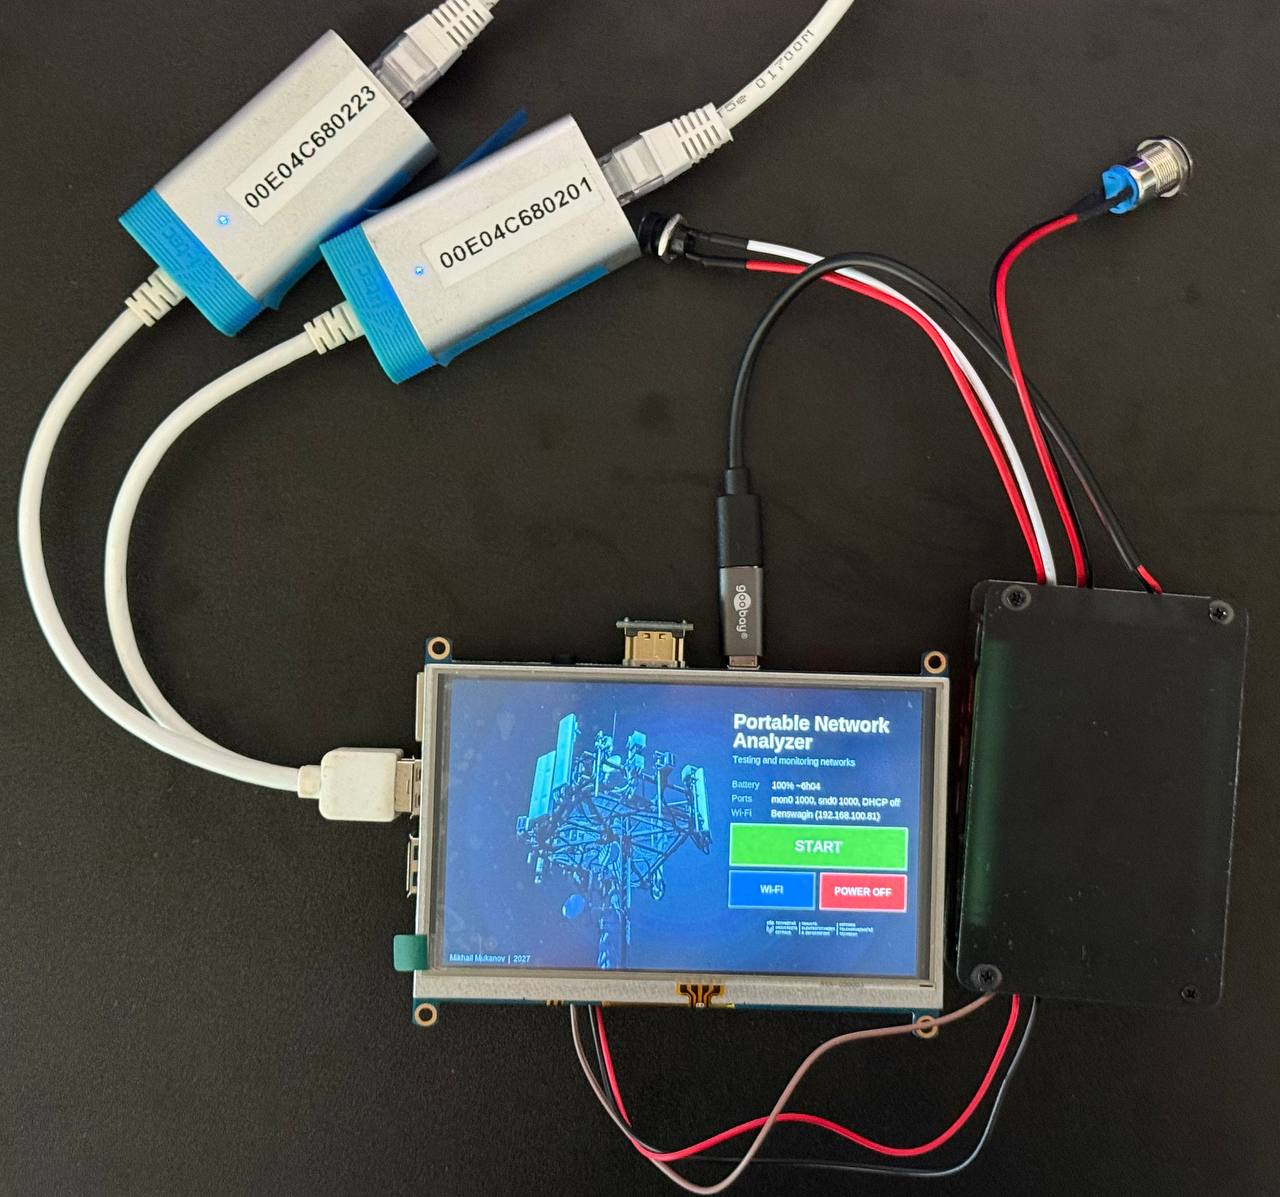
\includegraphics[width=0.78\textwidth]{device_prototype.jpg}};
\begin{scope}[x={(img.south east)},y={(img.north west)}]
\foreach \x/\y/\n in {0.22/0.86/1, 0.40/0.77/2, 0.53/0.30/3, 0.31/0.36/4, 0.585/0.50/5, 0.86/0.33/6, 0.90/0.88/7, 0.48/0.96/8}
  \node[circle,fill=callout,text=white,draw=white,line width=0.8pt,minimum size=1.5em,font=\bfseries\small] at (\x,\y) {\n};
\end{scope}
\end{tikzpicture}
\caption{Прибор целиком (корпуса пока нет)}
\end{figure}

\begin{callouts}
\item Адаптер USB--LAN с наклейкой \texttt{00E04C68\textbf{0223}}~--- это тестовый порт \textbf{SND}.
\item Адаптер с наклейкой \texttt{00E04C68\textbf{0201}}~--- тестовый порт \textbf{MON}. Оба адаптера~---
  Realtek RTL8153, гигабитные; их дал Nevlud.
\item Сенсорный экран 5\,дюймов, 800\,×\,480. Он \emph{резистивный}: нажимать надо уверенно, кончиком
  пальца или ногтем; у самого края экрана точность хуже, это свойство панели.
\item Под экраном~--- Raspberry Pi 3 Model B+ (сам компьютер). Сюда в USB-разъёмы вставлены адаптеры.
\item Питание входит в Raspberry Pi через переходник USB-C\,$\rightarrow$\,micro-USB.
\item Модуль питания с тремя аккумуляторами 18650 (Waveshare UPS 3S). От него прибор работает без
  розетки; полный разряд в тесте~--- 6\,ч\,43\,мин.
\item Кнопка включения питания (с фиксацией).
\item Патч-корд, которым MON и SND соединены между собой,~--- это «петля», стенд для проверки прибора
  самим собой.
\end{callouts}

Кроме двух тестовых портов у Raspberry Pi есть встроенный Wi-Fi. Через него прибор подключается к
обычной сети (дома~--- роутер, в лаборатории~--- точка доступа iPhone), и по нему можно зайти на прибор с
ноутбука по SSH. В тестах на тестовых портах Wi-Fi не участвует.

\begin{figure}[H]\centering
\begin{tikzpicture}[box/.style={draw,rounded corners,fill=gray!8,align=center,minimum height=1.1cm,
  font=\small},line width=0.7pt,node distance=0.9cm and 1.0cm]
\node[box,fill=teal!12,minimum width=3.6cm] (pi) {Raspberry Pi + экран\\(прибор)};
\node[box,left=1.4cm of pi,fill=blue!8] (mon) {адаптер \textbf{MON}\\\texttt{…02:01}};
\node[box,right=1.4cm of pi,fill=blue!8] (snd) {адаптер \textbf{SND}\\\texttt{…02:23}};
\node[box,below=1.3cm of mon] (net1) {розетка, коммутатор\\или ноутбук};
\node[box,below=1.3cm of snd] (net2) {второй конец\\или петля к MON};
\node[box,above=1.0cm of pi] (wifi) {точка доступа iPhone / домашний роутер\\$\rightarrow$ ноутбук по SSH};
\node[box,below=1.3cm of pi,fill=green!8] (bat) {модуль питания,\\3 аккумулятора};
\draw (mon) -- node[above,font=\scriptsize]{USB} (pi);
\draw (pi) -- node[above,font=\scriptsize]{USB} (snd);
\draw (mon) -- node[left,font=\scriptsize]{кабель RJ45} (net1);
\draw (snd) -- node[right,font=\scriptsize]{кабель RJ45} (net2);
\draw[decorate,decoration={snake,amplitude=1.2pt,segment length=6pt}] (pi) -- node[right,font=\scriptsize]{Wi-Fi} (wifi);
\draw[-{Latex}] (bat) -- node[right,font=\scriptsize]{5\,В} (pi);
\end{tikzpicture}
\caption{Как всё соединено}
\end{figure}

\section{Два порта: MON и SND}

\subsection{Зачем два порта}

У прибора два независимых тестовых порта. Названия условные: \textbf{MON} (monitor, «слушать») и
\textbf{SND} (sender, «отправлять»). На деле любой экран может работать с любым из них: внизу каждого
экрана есть две кнопки, ими и выбирают порт. Два порта нужны, чтобы:

\begin{itemize}
\item одним портом слать трафик, а другим его ловить и считать (генератор, измерение скорости на
  петле);
\item проверять две розетки или два сегмента, не переключая кабель;
\item проверять прибор самим собой: MON и SND соединены патч-кордом («петля»), и прибор становится
  своим собственным стендом.
\end{itemize}

\subsection{Почему порты не мешают друг другу}

Каждый порт живёт в своей отдельной «комнате» Linux~--- пространстве имён сети (network namespace,
netns). У каждой комнаты свои адреса, свои маршруты, своя таблица соседей. Между комнатами прибор сам
ничего не пересылает. Поэтому пакет с SND до MON может дойти \emph{только по кабелю}, как между двумя
разными компьютерами, а прибор, воткнутый в две разные сети, никогда не соединит их между собой. Это
главная техническая идея работы.

У каждого порта есть свои постоянные адреса для стенда:

\begin{center}
\begin{tabular}{llll}
\toprule
Порт & Комната (netns) & IPv4 & IPv6 \\
\midrule
MON (\texttt{mon0}) & \texttt{analyzer\_monitor} & 10.0.1.10/24 & fd00:1::10/64 \\
SND (\texttt{snd0}) & \texttt{analyzer\_sender} & 10.0.2.10/24 & fd00:2::10/64 \\
\bottomrule
\end{tabular}
\end{center}

Это разные подсети, поэтому на петле по IPv4 порты друг друга «не видят» (и прибор так прямо и
пишет), а по IPv6 видят всегда: у каждого порта есть адрес link-local (\texttt{fe80::…}), который
работает на любом проводе без настройки.

\subsection{Какой адаптер какой порт}

\begin{tcolorbox}[colback=gray!5,colframe=gray!60,boxrule=0.5pt,arc=2pt]
На наклейке адаптера напечатан его MAC-адрес. Последние четыре цифры видны на кнопках портов:

\begin{tabular}{lll}
наклейка \texttt{00E04C68\textbf{0201}} & $\rightarrow$ кнопка \btn{MON 02:01} & $\rightarrow$ порт \texttt{mon0} \\
наклейка \texttt{00E04C68\textbf{0223}} & $\rightarrow$ кнопка \btn{SND 02:23} & $\rightarrow$ порт \texttt{snd0} \\
\end{tabular}
\end{tcolorbox}

Привязка постоянная: адаптер \texttt{…0201} всегда MON, в какой бы USB-разъём его ни вставили, и
\texttt{…0223} всегда SND. Цифры на кнопке прибор читает из самого адаптера, а не из памяти.

Если вставить \textbf{другой} USB-LAN адаптер, прибор сам займёт им свободное место: например, если
адаптера \texttt{…0201} нет, через 3 секунды новый адаптер станет портом MON, и на кнопке появятся его
цифры. Когда «свой» адаптер с наклейкой вернётся, запасной уступит ему место. Запасные адаптеры, которым
места не досталось, перечислены на экране SYSTEM в строке \textbf{Spare ... not used}. Первые 30 секунд
после включения прибор ничего не переназначает~--- даёт своим адаптерам время определиться.

Мигать лампочкой по команде, чтобы найти адаптер, эти адаптеры не умеют (проверено). Самый быстрый
способ понять, где какой порт,~--- выдернуть кабель: на строке состояния точка этого порта станет
красной.

\section{Главное правило: прибор молчит, пока не нажмёшь}

Пока ты ничего не нажал, прибор ничего не отправляет в сеть, куда бы его ни воткнули. Отключено даже
то, что Linux обычно делает сам (запросы Router Solicitation при подключении кабеля). Любой активный
кадр уходит только по нажатию кнопки. Это сделано, чтобы прибор можно было спокойно втыкать в чужую
сеть, например в сеть кафедры.

\begin{center}
\small
\begin{tabularx}{\textwidth}{>{\raggedright}p{4.3cm}X}
\toprule
Кнопка & Что уходит в сеть \\
\midrule
\btn{AUTOTEST $\rightarrow$ START} & запрос адреса DHCP (адрес берётся примерно на 10\,с и возвращается), один RS (IPv6), 3 ping шлюзу, запрос DNS, одно TCP-соединение к www.vsb.cz:443 \\
\btn{PORT $\rightarrow$ LISTEN} & ничего, только слушает \\
\btn{PORT $\rightarrow$ HELLO} & один кадр LLDP с именем прибора \\
\btn{TRAFFIC} & ничего, только слушает \\
\btn{GENERATOR} & пакеты только на \emph{второй порт этого же прибора} \\
\btn{SPEED} & нагрузка iperf3; к адресу вне стенда~--- только после подтверждения \\
\btn{SCAN} & ARP по подсети порта, echo IPv6 всем соседям, Nmap к выбранной цели \\
\btn{IPv6 $\rightarrow$ RA SCAN} & один RS \\
\btn{PATH} & 4 ping к цели \\
\btn{DHCP / RA $\rightarrow$ TURN ON} & прибор \textbf{сам становится DHCP-сервером} и рассылает RA \\
\bottomrule
\end{tabularx}
\end{center}

\begin{warn}
\btn{DHCP / RA} включать только на стенде (петля, свой ноутбук) или в своей сети. В сети кафедры
прибор с включённым DHCP станет вторым DHCP-сервером и раздаст адреса чужим компьютерам. Перед тем как
воткнуть кабель в розетку лаборатории, проверь строку состояния: там должно быть серое
\textbf{DHCP off}. По умолчанию после включения DHCP всегда выключен.
\end{warn}

\section{Включение, приветствие, блокировка, выключение}

\subsection{Включение}

Нажми кнопку питания на модуле. Примерно через 36 секунд откроется приветственный экран. Рабочего стола
Linux нет: это «режим прибора», меню анализатора запускается само и само перезапускается, если вдруг
упадёт.

\shot[0.85]{ann/01_welcome.png}{Приветственный экран}

\begin{callouts}
\item \textbf{Battery}~--- заряд и примерное оставшееся время; на зарядке пишет \emph{charging} или
  \emph{AC}.
\item \textbf{Ports}~--- есть ли линк на портах и скорость (1000 = 1 Гбит/с), включён ли DHCP.
\item \textbf{Wi-Fi}~--- к какой сети подключён прибор и его адрес в ней (по этому адресу заходят
  по SSH).
\item \btn{START}~--- войти в главное меню.
\item \btn{WI-FI}~--- выбрать сеть Wi-Fi (раздел~\ref{sec:wifi}).
\item \btn{POWER OFF}~--- выключить. Нужно нажать \emph{дважды}: первое касание превращает кнопку в
  «TAP AGAIN TO CONFIRM», второе в течение 4 секунд выключает.
\end{callouts}

\subsection{Блокировка экрана}

Через 10 минут без касаний или по кнопке \btn{LOCK} на экране SYSTEM прибор блокируется: экран гаснет
(на светящейся подсветке дисплей пишет «No signal»~--- это нормально, подсветку программно не погасить).
Тесты при этом продолжают идти.

Первое касание погашенного экрана только будит его и ничего не нажимает. Появляется тот же
приветственный экран, но вместо START на нём \btn{UNLOCK}. Если ничего не нажать, через 30 секунд экран
снова погаснет.

\shot[0.6]{103_lock_screen.png}{Экран блокировки: нажми UNLOCK}

\subsection{Выключение и батарея}

Выключать только кнопкой \btn{POWER OFF} (на приветствии или на экране SYSTEM), а не выдёргиванием
питания: иначе можно повредить карту памяти. Если батарея сядет ниже 9,6\,В, прибор выключится сам,
аккуратно. Заряжать комплектным блоком 12,6\,В.

\section{Главный экран}

\shot[0.9]{ann/03_home_results.png}{Главный экран с итогами нескольких тестов}

Сверху на всех экранах одна и та же \textbf{строка состояния}:

\begin{callouts}
\item Название экрана (здесь~--- главный, NETWORK ANALYZER).
\item Порт \texttt{mon0}: \textcolor{green!60!black}{зелёная точка} и скорость~--- кабель подключён,
  линк есть; \textcolor{red}{красная точка} и \emph{down}~--- кабеля нет или другой конец выключен;
  \emph{mon0 --}~--- адаптер не вставлен.
\item То же для \texttt{snd0}.
\item \textbf{DHCP on} (оранжевым)~--- прибор раздаёт адреса; \textbf{DHCP off} (серым)~--- молчит.
\item Сеть Wi-Fi, к которой подключён прибор.
\item Время (часовой пояс Прага, синхронизация по интернету).
\item Батарея в процентах.
\end{callouts}

Ниже 12 \textbf{плиток}~--- функции прибора. Нажатие на плитку открывает её экран.

\begin{callouts}[start=8]
\item Название функции.
\item Коротко, что она умеет.
\item Итог последнего теста: \textcolor{green!60!black}{PASS}, \textcolor{orange}{WARN},
  \textcolor{red}{FAIL}, INFO, и главное число. Пока тест не запускали, там написано \emph{ready}.
\item Серые плитки с надписью \emph{not yet} (WATCH и RESULTS) ещё не сделаны и не нажимаются.
\end{callouts}

\section{Как устроен любой экран функции}

Все экраны функций построены по одному шаблону. Разобравшись с одним, понимаешь все.

\shot[0.9]{ann/22_autotest_done.png}{Шаблон экрана на примере AUTOTEST}

\begin{callouts}
\item Название экрана.
\item \textbf{Слово итога}~--- главный ответ теста (таблица ниже).
\item Пояснение к итогу с главным числом.
\item Рабочая область: у каждого экрана своё содержимое. У AUTOTEST это шаги теста, у других
  экранов~--- журнал, таблица или панели. Здесь~--- название шага.
\item Слово итога отдельного шага.
\item Подробности шага.
\item Граница рабочей области.
\item \btn{MON}~--- тест на порту MON. Выбранная кнопка синяя; под названием последние цифры MAC
  адаптера, как на наклейке.
\item \btn{SND}~--- тест на порту SND.
\item Главная кнопка действия. Пока тест идёт, она превращается в красную \btn{STOP}~--- ею тест можно
  остановить в любой момент.
\item Дополнительные кнопки (у каждого экрана свои).
\item \btn{BACK}~--- назад на главный экран. Всегда в одном и том же месте.
\end{callouts}

\begin{center}
\small
\begin{tabularx}{\textwidth}{lX}
\toprule
Слово & Что значит \\
\midrule
\textcolor{green!60!black}{\textbf{PASS}} & всё в порядке \\
\textcolor{orange}{\textbf{WARN}} & работает, но есть что-то подозрительное (полудуплекс, два DHCP-сервера, потери) \\
\textcolor{red}{\textbf{FAIL}} & не работает (нет линка, никто не ответил) \\
\textbf{SKIP} & шаг пропущен, и рядом написано почему (например, нет адреса~--- нечего пинговать) \\
\textbf{INFO} & просто сведения, без оценки \\
\textcolor{cyan!60!black}{\textbf{RUNNING}} & тест идёт, рядом секунды \\
\textbf{STOPPED} & тест остановлен кнопкой STOP \\
\textbf{BUSY} & на этом порту уже идёт другой тест: на одном порту одновременно только один тест \\
\textbf{IDLE} & ничего ещё не запускали \\
\bottomrule
\end{tabularx}
\end{center}

На экранах с журналом (SCAN, IPv6, PATH, DETAILS) справа две большие кнопки со стрелками вверх и вниз: они
листают журнал по страницам. Жестов (свайпов) прибор не понимает~--- только нажатия.

\textbf{Каждый результат сохраняется сам}: в папку \texttt{\textasciitilde/results/<дата>/} на приборе
пишется файл \texttt{<время>\_<скрипт>\_<порт>.json} с итогом, временем, отметкой, синхронизированы ли
часы, и контрольной суммой программы. Это данные для таблиц в работе. Достать их можно по SSH
(раздел~\ref{sec:results}).

% -----------------------------------------------------------------------------------------------------
\section{AUTOTEST~--- проверка розетки одной кнопкой}

Главная функция для показа. Втыкаешь кабель в розетку, выбираешь порт, жмёшь \btn{START}~--- и прибор за
6–10 секунд проходит шесть шагов сверху вниз. Это то же, что делают коммерческие тестеры (Fluke
LinkRunner и подобные).

\shot[0.72]{20_autotest_idle.png}{AUTOTEST до запуска: под каждым шагом написано, что он проверяет}
\shot[0.72]{21_autotest_running.png}{Идёт прогон: шаг 2 из 6, дальше «waiting»}

\begin{center}
\small
\begin{tabularx}{\textwidth}{>{\bfseries}lX}
\toprule
Шаг & Что делает и как читать \\
\midrule
LINK & Есть ли связь по кабелю, скорость, дуплекс, автосогласование (как экран PORT). FAIL~--- нет линка, и тогда все остальные шаги SKIP. \\
DHCPv4 & Рассылает запрос «кто даст адрес?» и 4 секунды собирает \emph{все} ответы. Один сервер~--- PASS, два и больше~--- \textbf{WARN} с адресами всех (в сети чужой роутер~--- частая причина проблем). Никто не ответил~--- FAIL. Потом берёт предложенный адрес, а в конце прогона \textbf{возвращает} его серверу (даже если нажать STOP). Время ответа в мс. \\
IPv6 & Просит у роутеров объявление (RS) и разбирает ответ (RA): префикс, флаги M/O/A, получил ли порт свой адрес SLAAC. Нет ответа~--- INFO: «в этой сети нет IPv6». \\
GATEWAY & Три ping шлюзу, который дал DHCP, и роутеру IPv6. Отвечает на ARP, но не на ping~--- WARN (ping закрыт). \\
DNS & Спрашивает у DNS-сервера сети адрес \texttt{www.vsb.cz} (A и AAAA), время ответа. \\
TARGETS & Короткое TCP-соединение к \texttt{www.vsb.cz} на порт 443 (как начало открытия сайта, но без загрузки страницы). \\
\bottomrule
\end{tabularx}
\end{center}

Общий итог сверху: если хоть один шаг FAIL~--- FAIL, если есть WARN~--- WARN, иначе PASS. SKIP и INFO итог
не портят.

\textbf{На петле} (снимок в разделе 6) шлюз, DNS и сайт честно пропущены (SKIP): DHCP-сервер прибора
нарочно раздаёт только адрес, без шлюза и DNS, чтобы ноутбук, подключённый к прибору, не отправил в
него весь свой интернет. А вот \textbf{в настоящей сети} проходят все шесть шагов~--- так было дома через
роутер провайдера:

\shot[0.72]{autotest_home.png}{Прогон в настоящей сети (дома, 04.10): PASS по всем шагам за 6,9\,с.
Снимок сделан до появления MAC на кнопках портов}

\btn{DETAILS}~--- полный журнал прогона: все ответы DHCP с адресами серверов, флаги RA, ответы ping и DNS.
Пригодится, если надо понять, \emph{почему} шаг получил WARN или FAIL.

\shot[0.72]{23_autotest_details.png}{Страница DETAILS}

\begin{tip}
Интересная находка для рассказа: многие роутеры (на dnsmasq) перед выдачей адреса пингуют его и ждут
3 секунды. Окно ожидания в ТЗ было ровно 3 секунды и такие ответы ловило случайно~--- поэтому окно
сделано 4 секунды. На стенде это хорошо видно: «offer … in 3048 ms».
\end{tip}

% -----------------------------------------------------------------------------------------------------
\section{PORT~--- линк и кто на другом конце кабеля}

\shot[0.9]{ann/13_port_lldp.png}{PORT: слева линк, справа сосед (здесь~--- второй порт самого прибора)}

\begin{callouts}
\item \textbf{LINK}~--- что сообщает сам адаптер. Обновляется само при открытии экрана и когда кабель
  втыкают или выдёргивают (меньше чем за 2 секунды). Ничего в сеть не шлёт.
\item \textbf{NEIGHBOUR / SWITCH}~--- кто на другом конце, после \btn{LISTEN}.
\item Выбор порта (с цифрами MAC).
\item \btn{CHECK}~--- перечитать адаптер прямо сейчас (и сохранить результат).
\item \btn{LISTEN}~--- слушать до 65 секунд, что сообщает о себе коммутатор. Ничего не отправляет.
\item \btn{HELLO}~--- отправить один свой кадр LLDP («я тут: raspberrypi, порт mon0»).
\end{callouts}

Строки левой панели:

\begin{center}
\small
\begin{tabularx}{\textwidth}{>{\bfseries}lX}
\toprule
Link & есть ли линк, скорость (Mb/s) и дуплекс (full~--- в обе стороны одновременно, half~--- по очереди, это плохо) \\
Autoneg & автосогласование: обе стороны сами договорились о скорости (\emph{on, both sides}~--- норма; \emph{other end fixed}~--- на другом конце скорость задана жёстко) \\
Partner & какие режимы умеет \emph{другой конец кабеля}: \texttt{1000F}~--- 1000 Мбит/с full duplex, \texttt{100H}~--- 100 half и т.\,д. Прибор узнаёт это из автосогласования, без всякого LLDP \\
This port & какие режимы предлагает сам адаптер прибора \\
Link drops & сколько раз пропадал линк: новых с прошлой проверки и всего с включения \\
Errors & ошибки приёма и передачи с прошлой проверки; \emph{missed}~--- кадры, которые адаптер не успел принять \\
Adapter, MAC & драйвер, прошивка и MAC адаптера \\
\bottomrule
\end{tabularx}
\end{center}

Итог: \textbf{FAIL}~--- нет линка; \textbf{WARN}~--- полудуплекс, или обе стороны умеют 1000, а линк встал
на 100 (обычно виноват кабель, в котором работают не все 4 пары), или другой конец с жёсткой скоростью;
иначе \textbf{PASS}.

\subsection{LISTEN: имя коммутатора, порт, VLAN}

Управляемые коммутаторы сами периодически рассказывают о себе: по протоколу \textbf{LLDP} (стандарт IEEE,
раз в 30 секунд) или \textbf{CDP} (Cisco, раз в 60 секунд). \btn{LISTEN} ловит эти кадры и показывает:

\begin{center}
\small
\begin{tabularx}{\textwidth}{>{\bfseries}lX}
\toprule
Name & имя коммутатора \\
Port & номер или имя порта коммутатора, куда воткнут кабель, и его описание \\
VLAN & в какой VLAN этот порт (если коммутатор это сообщает) \\
Mgmt IP & адрес управления коммутатора \\
Model & модель или версия ПО \\
Chassis & идентификатор коммутатора (обычно MAC) \\
TTL & сколько секунд эти сведения считаются свежими \\
Also & что ещё услышано: STP (за розеткой коммутатор), LACP (порт в агрегации), кадры с метками VLAN \\
\bottomrule
\end{tabularx}
\end{center}

Прослушка заканчивается сама, как только услышан коммутатор, или через 65 секунд. Если ничего не
услышано~--- «nothing heard»: LLDP и CDP на этом коммутаторе выключены. \textbf{Это тоже результат}, его
надо записать (Nevlud предупреждал, что в лаборатории они скорее выключены). Строка Also всё равно
может показать STP~--- значит, за розеткой коммутатор.

\shot[0.62]{11_port_listening.png}{Идёт прослушка: «listening, sending nothing», полоска~--- прошедшее время}

\subsection{HELLO и как показать LLDP дома}

\btn{HELLO} отправляет один кадр LLDP с именем прибора, портом и адресом. Коммутатор запомнит прибор
на 120 секунд и покажет его у себя в списке соседей; некоторые коммутаторы в ответ сразу присылают свой
LLDP. Дома коммутатора нет, поэтому LLDP показывают на петле:

\begin{enumerate}
\item На экране PORT выбери \btn{MON}, нажми \btn{LISTEN}.
\item Выбери \btn{SND}, нажми \btn{HELLO}. На SND появится «Sent LLDP at …, kept 120 s».
\item Выбери \btn{MON}: справа будет «NEIGHBOUR this device, snd0, LLDP» с именем raspberrypi и
  портом snd0 (снимок в начале раздела).
\end{enumerate}

\shot[0.62]{12_port_hello.png}{После HELLO на порту SND}

% -----------------------------------------------------------------------------------------------------
\section{TRAFFIC~--- живой трафик}

Пассивный анализатор: показывает, что идёт по кабелю выбранного порта. Ничего не отправляет.

\shot[0.9]{ann/70b_traffic_live.png}{TRAFFIC во время захвата}

\begin{callouts}
\item Пакетов в секунду.
\item Мегабит в секунду.
\item Средний размер пакета.
\item Сколько разных адресов (хостов) замечено.
\item \textcolor{red}{LIVE}~--- захват идёт; порт и длительность.
\item Полоса долей протоколов.
\item Те же доли числами: TCP, UDP, ICMP, ICMPv6, ARP, прочее (под каждым~--- число пакетов).
\item \textbf{TOP TALKERS}~--- кто больше всех отправил (по байтам).
\item \textbf{PACKETS}~--- лента последних пакетов: время, протокол, размер, откуда\,>\,куда, краткий разбор.
\item Какой фильтр сейчас включён.
\item \btn{START} / \btn{STOP}~--- начать или закончить захват.
\item \btn{PAUSE}~--- «заморозить» последние 200 пакетов и листать их (счёт при этом идёт дальше).
\item \btn{FILTER}~--- оставить только нужный трафик.
\item \btn{SAVE}~--- сохранить захват в \texttt{\textasciitilde/results}: файл PCAP (открывается в
  Wireshark), CSV и итог JSON.
\end{callouts}

Захват пишется во временную память до 20\,МБ. Если переключить порт во время захвата, захват
перезапустится на новом порту.

\shot[0.62]{71_traffic_paused.png}{PAUSED: последние пакеты, по 5 на странице; листать кнопками PAGE}

Нажатие на пакет в PAUSED открывает его разбор по уровням: Ethernet (MAC-адреса), IPv4/IPv6, TCP/UDP/ICMP
и т.\,д.~--- как в Wireshark, только крупно. \btn{PREV} / \btn{NEXT}~--- соседние пакеты, \btn{FILTER THIS
HOST}~--- сразу включить фильтр по адресу этого пакета.

\shot[0.62]{72_traffic_packet.png}{PACKET: разбор одного пакета (TCP SYN на порт 9)}

\btn{FILTER} открывает 9 готовых фильтров: ALL (всё), TCP, UDP, ICMP, ARP, DHCP, ND/RA (служебные
сообщения IPv6), DNS и HOST (выбрать адрес из TOP TALKERS). Фильтр работает прямо в ядре Linux (BPF):
ненужные пакеты даже не доходят до программы, поэтому прибор успевает больше.

\shot[0.62]{73_traffic_filter.png}{FILTER: выбор фильтра}

\begin{tip}
Самая наглядная демонстрация двух портов: на MON запусти TRAFFIC, а на SND~--- SPEED (UDP, IPv6, TIME
30\,s). TRAFFIC покажет около 8\,750 пакетов в секунду и около 104 Мбит/с, а SPEED в конце отчитается о
8\,753 пакетах в секунду. Один порт генерирует, второй независимо считает~--- и числа совпадают.
\end{tip}

\shot[0.72]{76_traffic_with_speed.png}{TRAFFIC на MON, пока SPEED шлёт UDP с SND}

% -----------------------------------------------------------------------------------------------------
\section{GENERATOR~--- генератор пакетов}

Шлёт пакеты выбранного типа с одного порта на \emph{второй порт этого же прибора} и считает, сколько
дошло. В чужую сеть генератор не шлёт никогда.

\shot[0.9]{ann/82_generator_done.png}{GENERATOR: 1000 пакетов ICMPv6 отправлено с SND, все 1000 приняты на MON}

\begin{callouts}
\item Тип пакета: \textbf{ICMP} (ping IPv4), \textbf{ICMPv6} (ping IPv6), \textbf{UDP} (на порт 9),
  \textbf{TCP SYN} (запрос соединения на порт 9), \textbf{ARP} (запрос «чей это адрес»), \textbf{RS}
  (запрос роутера IPv6).
\item \btn{COUNT}~--- сколько: 100, 1000, 10\,000 или «until STOP» (пока не остановишь). Каждое нажатие
  переключает на следующее значение.
\item \btn{RATE}~--- скорость: 10, 100, 1000 пакетов в секунду или max.
\item \btn{SIZE}~--- размер кадра: минимальный, 128, 512 или 1514 байт (только для ICMP, ICMPv6, UDP).
\item \btn{TO}~--- куда: второй порт прибора, адрес подставляется сам (нажатие показывает адрес и MAC).
\item Сколько отправлено.
\item Сколько принято на втором порту (там в это время работает свой счётчик).
\item Полоска хода.
\item Порт-отправитель: выбранный (здесь SND), принимает всегда другой.
\item \btn{SEND}~--- начать (во время отправки~--- \btn{STOP}).
\end{callouts}

Итог \textbf{PASS}, если принято столько же, сколько отправлено; \textbf{WARN} с числом потерь, если
меньше. Перед отправкой прибор несколько секунд готовит пакеты (надпись «preparing packets»). Итог
сохраняется; при повторном входе на экран числа счётчиков сбрасываются, а слово итога сверху остаётся.

% -----------------------------------------------------------------------------------------------------
\section{SPEED~--- пропускная способность (iperf3)}

\shot[0.9]{ann/91_speed_done.png}{SPEED: UDP по IPv6 на петле, 100 Мбит/с без потерь}

\begin{callouts}
\item \btn{TCP} / \btn{UDP}: TCP меряет, сколько реально пропускает соединение; UDP шлёт с заданной
  скоростью и показывает потери и джиттер.
\item \btn{IPv4} / \btn{IPv6}.
\item \btn{RATE}~--- скорость для UDP: 10, 100, 200, 400 Мбит/с или max (у TCP всегда max).
\item \btn{TIME}~--- длительность: 5, 10 или 30 секунд.
\item \btn{DIRECTION}~--- в какую сторону: прибор\,$\rightarrow$\,хост или хост\,$\rightarrow$\,прибор.
\item \btn{TO}~--- куда: \emph{auto}~--- прибор находит соседа сам; на петле сам поднимает приёмник на
  втором порту.
\item Результат: пропускная способность (Мбит/с), пакетов в секунду, потери, джиттер (разброс задержки).
\item Куда мерили, загрузка процессора, температура чипа, не было ли перегрева/просадки питания
  (такой прогон получает WARN).
\item \btn{START}.
\item \btn{SWEEP}~--- развёртка по размерам кадра.
\item \btn{SERVER}~--- сделать прибор сервером iperf3, чтобы мерил другой компьютер.
\end{callouts}

\textbf{На петле выбирай IPv6}: по IPv4 порты в разных подсетях, и прибор так и пишет:

\shot[0.62]{91b_speed_fail_v4.png}{IPv4 на петле: FAIL с объяснением «use v6»}

\textbf{Какие числа ожидать.} У Raspberry Pi 3B+ все USB-порты и Ethernet висят на одной шине USB~2.0,
официальный потолок~--- около 300 Мбит/с, хотя линк показывает 1000. К внешнему ноутбуку прибор
выдаёт около 275 Мбит/с, а на петле около 150 Мбит/с: кадр проходит шину дважды (уходит с одного адаптера и
приходит на другой). Это ограничение платформы, и в работе оно честно записано.

\shot[0.72]{92_speed_sweep.png}{SWEEP: UDP по 7 размерам кадра (RFC 2544), около 80 секунд}

\btn{SWEEP} прогоняет UDP по семи размерам кадра из стандарта RFC~2544 (для IPv6 начиная с 82 байт) по
10 секунд и строит таблицу: Мбит/с, пакеты в секунду, потери, джиттер. Видно главное: мелкими кадрами
прибор шлёт больше пакетов, но меньше мегабит. Таблица сохраняется в CSV и JSON.

\btn{SERVER} запускает на выбранном порту сервер iperf3 и пишет команды, которые надо набрать на
другом компьютере (\texttt{iperf3 -c 10.0.1.10}). Остановить~--- \btn{STOP}.

\shot[0.62]{93_speed_server.png}{SERVER: прибор ждёт клиента iperf3}

\begin{warn}
Нагрузочные тесты (стандарт RFC~2544) нельзя гонять в рабочей сети~--- это прямо сказано в RFC~6815.
Поэтому если цель не из адресов стенда, SPEED показывает предупреждение и запускается только по
повторному нажатию \btn{START} в течение 6 секунд, а SWEEP вне стенда не запускается вовсе. В сети
кафедры SPEED не запускай~--- только к своему ноутбуку.
\end{warn}

% -----------------------------------------------------------------------------------------------------
\section{SCAN~--- кто есть в сети}

\shot[0.9]{ann/43_scan_nmap.png}{SCAN после Nmap}

\begin{callouts}
\item \textbf{Nmap target}~--- цель для Nmap. Нажатие открывает список: найденные цели, шлюз Wi-Fi,
  адреса стенда, или клавиатуру для ввода адреса.
\item \btn{GATEWAY}~--- взять целью шлюз сети Wi-Fi.
\item \btn{via test port} / \btn{via Wi-Fi}~--- через что сканировать: тестовый порт или Wi-Fi.
\item Журнал.
\item Листать журнал.
\item \btn{ARP}~--- опросить по IPv4 все адреса подсети порта (10.0.1.0/24 для MON): кто ответит.
\item \btn{NEIGHBORS}~--- найти соседей по IPv6 (один запрос всем, \texttt{ff02::1}) и по ARP; для
  каждого соседа прибор вычисляет его адрес из MAC (EUI-64) и проверяет его ping'ом. Найденное
  запоминается и подставляется в PATH и SPEED.
\item \btn{NMAP}~--- проверить 100 самых популярных портов цели и узнать службы (до 30 секунд).
\end{callouts}

\shot[0.62]{41_scan_target.png}{Выбор цели для Nmap}
\shot[0.62]{42_scan_keypad.png}{Клавиатура для ввода адреса (цифры, a–f, точка, двоеточие)}

\begin{warn}
Nmap и ARP-опрос в чужой сети запускать только с разрешения: сканирование портов администратор
может принять за атаку.
\end{warn}

% -----------------------------------------------------------------------------------------------------
\section{IPv6~--- аудит объявлений роутеров}

\btn{RA SCAN} отправляет один запрос роутерам (RS), 5 секунд слушает ответы (RA) и разбирает каждый:
флаги M (адреса через DHCPv6), O (прочие настройки через DHCPv6), A (можно строить адрес самому,
SLAAC), префикс, время жизни, MTU. Каждый роутер помечен: \emph{LOCAL TX}~--- отправил этот же порт,
\emph{OWN DEVICE}~--- второй порт прибора, \emph{FOREIGN}~--- чужой роутер. Ниже~--- проверки по стандартам
с пометками OK, INFO, WARN, ALERT.

\shot[0.72]{50_ipv6_ra.png}{RA SCAN на петле (DHCP/RA включён на втором порту)}

Итог: \textbf{PASS}~--- роутер есть, это прибор; \textbf{WARN}~--- есть чужой роутер; \textbf{INFO}~--- роутеров
нет. На стенде чужой роутер означает проблему, а \textbf{в сети кафедры роутер и должен быть чужим}
(FOREIGN)~--- это нормально.

% -----------------------------------------------------------------------------------------------------
\section{PATH~--- ping}

\btn{PING v4} и \btn{PING v6}~--- 4 ping к цели. Если в SCAN цель найдена, используется она, иначе прибор
ищет соседа сам (запись DHCP, таблица соседей, запрос всем). Если не ответили, прибор объясняет почему:
«хост на кабеле есть, но ping закрыт» или «хоста нет», а на петле по IPv4~--- что порты в разных сетях.

\shot[0.62]{60_path_v6.png}{PING v6 на петле: 4 из 4, 1,1\,мс}

% -----------------------------------------------------------------------------------------------------
\section{DHCP / RA~--- раздавать адреса на стенде}

\btn{TURN ON} включает на \emph{обоих} портах DHCP-сервер и рассылку RA; \btn{TURN OFF} выключает. Каждый
порт раздаёт один адрес (10.0.1.20 на MON, 10.0.2.20 на SND), без шлюза и DNS, а RA говорит «я не
маршрутизатор по умолчанию». Нужно, чтобы на стенде ноутбук или другое устройство получило адрес от
прибора.

\begin{figure}[H]\centering
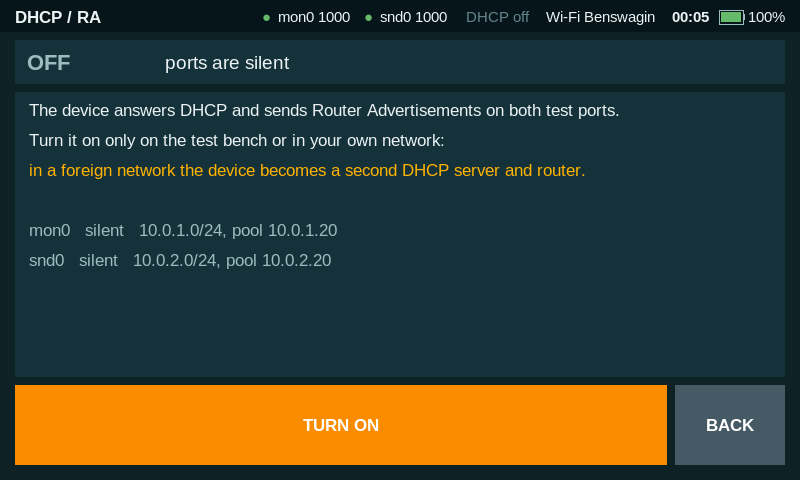
\includegraphics[width=0.48\textwidth]{30_dhcp_off.png}\hfill
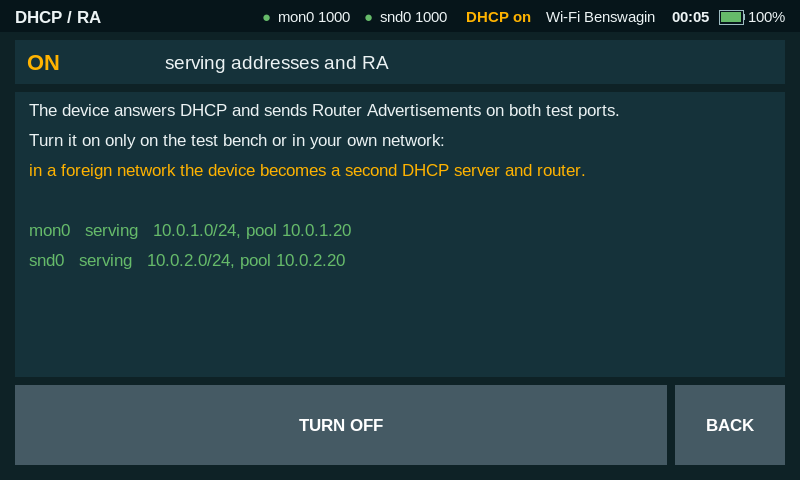
\includegraphics[width=0.48\textwidth]{31_dhcp_on.png}
\caption{DHCP / RA выключен (слева) и включён (справа)}
\end{figure}

Помни предупреждение из раздела 3: в чужой сети не включать.

% -----------------------------------------------------------------------------------------------------
\section{SYSTEM~--- сведения о приборе}

\shot[0.72]{100_system.png}{SYSTEM}

Строки: Wi-Fi и адрес, батарея (процент, напряжение, ток, на зарядке или нет), температура чипа и
\texttt{throttled} (должно быть \texttt{0x0}: нет перегрева и просадки питания), время работы, часы, MAC и
адрес каждого порта, свободные запасные адаптеры (Spare).

Кнопки: \btn{WI-FI}~--- выбор сети; \btn{LOCK}~--- заблокировать экран; \btn{DESKTOP}~--- выйти на рабочий стол
Linux (вернуться~--- выйти из сеанса через меню, анализатор запустится сам); \btn{CLEAR RESULTS}~--- стереть
надписи итогов на плитках и журналы экранов (найденные цели и идущий тест не трогает, файлы
результатов не удаляет); \btn{POWER OFF}~--- выключить (тоже двумя касаниями).

\begin{warn}
\btn{DESKTOP} на показе лучше не нажимать: рабочий стол на маленьком экране выглядит как «малина с
программой», а не как прибор.
\end{warn}

% -----------------------------------------------------------------------------------------------------
\section{Wi-Fi}\label{sec:wifi}

\shot[0.9]{ann/101_wifi.png}{Окно Wi-Fi}

\begin{callouts}
\item К какой сети подключён прибор и его адрес.
\item Сеть в списке: имя, состояние (\emph{connected}~--- подключён, \emph{saved}~--- пароль сохранён,
  \emph{secured}~--- с паролем). Нажатие выбирает сеть.
\item Сила сигнала.
\item Листать список (по 4 сети на странице).
\item \btn{RESCAN}~--- искать сети заново.
\item \btn{CONNECT}~--- подключиться к выбранной: сохранённая и открытая сеть подключаются сразу, для
  новой появится экранная клавиатура для пароля (\btn{SHIFT}~--- заглавные, \btn{?123}~--- цифры и
  символы).
\item \btn{DISCONNECT}~--- отключиться.
\item \btn{CLOSE}~--- закрыть окно.
\end{callouts}

В лаборатории своего Wi-Fi у прибора нет~--- включи точку доступа на iPhone: она в приборе уже сохранена
и подключается без пароля.

\section{Где лежат результаты}\label{sec:results}

Всё сохраняется на приборе в \texttt{/home/muk0015/results/<дата>/}. Скопировать на ноутбук можно
так (ноутбук в той же сети Wi-Fi, что и прибор):

\begin{verbatim}
scp -r malina:results/20261006 .
\end{verbatim}

Экспорт на флешку кнопкой (плитка RESULTS) ещё не сделан. Можно и просто попросить меня в сессии Claude
Code: я скопирую результаты и сниму экраны по SSH.

% =====================================================================================================
\part{Лаборатория EB215}

\section{Подготовка дома, накануне}

\begin{itemize}
\item Зарядить прибор до 100\,\% (на SYSTEM: \emph{100 \%, on charger}). Батареи хватает на 6+ часов.
\item На SYSTEM проверить \texttt{throttled=0x0}.
\item Убедиться, что \textbf{DHCP off}.
\item Взять с собой:
  \begin{itemize}
  \item прибор и блок питания 12,6\,В;
  \item оба адаптера с наклейками (уже на приборе) и запасные адаптеры от ноутбука;
  \item 2–3 патч-корда, один подлиннее (до розетки или стойки);
  \item ноутбук Acer (на нём уже стоит iperf3 и лежат файлы \texttt{analyzer\_firewall\_ON.cmd} /
    \texttt{\_OFF.cmd} на рабочем столе);
  \item iPhone для точки доступа.
  \end{itemize}
\item Перед уходом один раз на петле: GENERATOR (ICMPv6, SND) $\rightarrow$ PASS 1000/1000. Прибор жив.
\end{itemize}

\section{Порядок проверок в лаборатории}

Каждый шаг: что сделать, что должно получиться, что записать. Результаты сохраняются сами.

\subsection*{Шаг 0. Включить и подключить Wi-Fi}

Включи точку доступа на iPhone, включи прибор, на приветствии \btn{WI-FI} $\rightarrow$ выбрать iPhone
$\rightarrow$ \btn{CONNECT}. Ноутбук подключи к той же точке. Тогда на ноутбуке работает \texttt{ssh malina}
(если имя не находится~--- адрес прибора виден на приветствии в строке Wi-Fi), и я в сессии Claude Code
могу снимать экраны и забирать результаты.

\subsection*{Шаг 1. Проверить «DHCP off»}

Строка состояния: серое \textbf{DHCP off}. Если оранжевое \textbf{DHCP on}~--- плитка \btn{DHCP / RA}
$\rightarrow$ \btn{TURN OFF}. Только после этого кабель в розетку.

\subsection*{Шаг 2. Розетка сети кафедры (с разрешения Nevlud'а, он его дал)}

Кабель от адаптера \textbf{MON} (\texttt{…0201}) в розетку.

\begin{enumerate}
\item \textbf{PORT}, порт MON. Ожидаем: линк 1000 full (или 100, если розетка стоверная), строка
  Partner~--- что умеет порт коммутатора. Нажми \btn{CHECK}~--- результат сохранится.
\item \btn{LISTEN}, ждать до 65 секунд. Варианты: имя коммутатора и порт (LLDP/CDP) или «nothing heard».
  Оба варианта записываем. Посмотри строку Also: STP значит, что за розеткой коммутатор.
\item \textbf{AUTOTEST}, порт MON, \btn{START}. Это и есть главный пункт: прогон в настоящей сети
  кафедры. Ожидаем адрес от DHCP-сервера кафедры, шлюз, DNS, www.vsb.cz. Если WARN «2 servers»~--- в сети
  два DHCP-сервера, это настоящая находка, сфотографируй экран.
\item \textbf{IPv6}, \btn{RA SCAN}: роутер кафедры будет FOREIGN~--- в чужой сети это нормально. Если RA
  нет~--- в сети кафедры нет IPv6, тоже результат.
\item \textbf{TRAFFIC}, порт MON, \btn{START}, 30–60 секунд, потом \btn{SAVE}. В чужой сети к прибору
  прилетает только широковещательный и групповой трафик (ARP, STP, IPv6 ND, mDNS и т.\,п.)~--- видно,
  чем «шумит» сеть.
\end{enumerate}

\subsection*{Шаг 3. Коммутатор в стойке (MikroTik или Cisco), вместе с Nevlud'ом}

Кабель от MON в свободный порт коммутатора.

\begin{enumerate}
\item \textbf{PORT}: линк, режимы партнёра.
\item \btn{LISTEN}. Если коммутатор молчит~--- \btn{HELLO}, потом ещё раз \btn{LISTEN}.
\item Если у Nevlud'а есть доступ к коммутатору, попроси показать его список соседей: прибор после HELLO
  виден там 120 секунд как \emph{raspberrypi}, порт mon0 (MikroTik: \emph{IP $\rightarrow$ Neighbors};
  Cisco: \texttt{show lldp neighbors}). Это эффектная проверка «с двух сторон».
\item Если порт в VLAN, LLDP сообщит его номер (строка VLAN); если на порту ходят кадры с метками
  VLAN~--- они будут в строке Also.
\end{enumerate}

Настройки коммутатора сам не меняй~--- это делает Nevlud или администратор.

\subsection*{Шаг 4. Ноутбук: измерение скорости}

\begin{warn}
Сначала \textbf{выдерни MON из розетки кафедры}. DHCP включается на обоих портах сразу, и прибор не
должен раздавать адреса в сеть кафедры.
\end{warn}

\begin{enumerate}
\item Ноутбук кабелем к адаптеру \textbf{SND} (\texttt{…0223}) или прямо в его сетевой разъём.
\item \btn{DHCP / RA} $\rightarrow$ \btn{TURN ON}. Ноутбук получит адрес 10.0.2.20.
\item На ноутбуке двойной щелчок по \texttt{analyzer\_firewall\_ON.cmd} (разрешает iperf3 и ping), затем в
  терминале \texttt{iperf3 -s}.
\item На приборе \textbf{SPEED}, порт SND, TCP, IPv4, \btn{START}. Ожидаем около 275 Мбит/с.
\item Можно и наоборот: на приборе \btn{SERVER}, на ноутбуке \texttt{iperf3 -c 10.0.2.10}.
\item После: \btn{TURN OFF} DHCP, на ноутбуке \texttt{analyzer\_firewall\_OFF.cmd}.
\end{enumerate}

\subsection*{Шаг 5. Фото для работы}

Сфотографируй прибор, подключённый к компьютеру или коммутатору в лаборатории: это «второе фото» для
раздела о реализации (можно заменить им старое \texttt{lab\_connection.jpg}).

\subsection*{Что должно остаться после лаборатории}

Файлы в папке результатов за этот день: \texttt{port\_info}, \texttt{l2\_listen}, \texttt{autotest},
\texttt{ra\_audit}, захват \texttt{traffic} (PCAP), \texttt{perf\_test}~--- всё в сети кафедры. Плюс фото
экрана, если было что-то необычное, и фото прибора. Эти файлы пойдут в раздел о результатах.

\section{Сценарий показа Nevlud'у (10–15 минут)}

Порядок от общего к частному. Каждый пункт~--- что сделать и что примерно сказать своими словами.

\begin{enumerate}[label=\textbf{\arabic*.},leftmargin=1.6em]
\item \textbf{Прибор целиком.} Показать прибор, батарею, кнопку питания, два адаптера с наклейками.
  Включить и дождаться приветствия.
  \begin{say}
  Это самостоятельный прибор: включается кнопкой, через полминуты открывает меню на сенсорном
  экране, ноутбук не нужен. От аккумуляторов работает больше шести часов, в тесте разряда было 6\,ч
  43\,мин, при разряде выключается сам.
  \end{say}
\item \textbf{Главный экран.} Двенадцать функций, строка состояния, цифры MAC на кнопках портов. Можно
  показать подмену: вынуть адаптер \texttt{…0201}, вставить запасной~--- через 3 секунды он стал MON.
  \begin{say}
  Порты изолированы через network namespaces: у каждого свои адреса и маршруты, между ними пакет
  проходит только по кабелю. Поэтому одним портом можно генерировать, а другим независимо анализировать.
  \end{say}
\item \textbf{Петля: генератор и анализатор вместе.} На MON запустить TRAFFIC, на SND~--- SPEED (UDP,
  IPv6, 30\,s). Показать, что TRAFFIC видит около 8\,750 пак/с и около 104 Мбит/с, а SPEED в конце пишет 8\,753
  пак/с. Потом GENERATOR (ICMPv6, SND) $\rightarrow$ 1000/1000.
  \begin{say}
  Анализатор считает независимо от генератора, и числа совпадают. Разбор пакетов я сверил с tshark:
  781 поле на 58 кадрах, расхождений нет.
  \end{say}
\item \textbf{PORT.} Линк, режимы партнёра, LLDP на петле (HELLO с SND, LISTEN на MON), потом~--- на
  коммутаторе в стойке.
  \begin{say}
  Режимы партнёра прибор видит без LLDP~--- из автосогласования. А LLDP и CDP говорят имя коммутатора,
  порт и VLAN. Если они выключены, прибор так и пишет, и по STP видно, что за розеткой коммутатор.
  \end{say}
\item \textbf{AUTOTEST} в розетке кафедры (или показать домашний прогон, если розетки нет).
  \begin{say}
  Одна кнопка отвечает, что с розеткой: линк, DHCP, IPv6, шлюз, DNS, доступность сайта. Адрес берётся
  только на время теста и возвращается серверу. Если в сети два DHCP-сервера, будет WARN с адресами
  обоих.
  \end{say}
\item \textbf{SPEED и SWEEP} (можно показать готовую таблицу развёртки).
  \begin{say}
  Линк гигабитный, но у Raspberry Pi 3B+ всё на одной шине USB~2.0: к ноутбуку около 275 Мбит/с, на
  петле около 150, потому что кадр проходит шину дважды. Это честное ограничение платформы.
  \end{say}
\item \textbf{IPv6}: RA SCAN, SCAN $\rightarrow$ NEIGHBORS (адрес соседа вычисляется из MAC и проверяется).
\item \textbf{Что дальше:} корпус (3D-печать на кафедре, контакт Ing. Hejduk), функции WATCH и RESULTS с
  экспортом на флешку, калибровка экрана, затем текст.
\end{enumerate}

\section{Вопросы, которые может задать Nevlud}

\begin{description}[leftmargin=0pt,style=nextline,itemsep=0.5em]
\item[Зачем два порта и network namespaces?]
  Чтобы один порт мог слать трафик, а второй независимо его ловить, и чтобы прибор в двух сетях не
  соединял их. У каждого порта своя изолированная сетевая «комната»: адреса, маршруты, соседи.
\item[Почему 150 или 275 Мбит/с, если линк 1000?]
  Ethernet и USB у Raspberry Pi 3B+ на одной шине USB 2.0, официальный потолок около 300 Мбит/с
  (Product Brief). 1000~--- это скорость, о которой договорился кабель, а не то, что успевает компьютер.
\item[Зачем AutoTest берёт адрес у DHCP?]
  Без своего адреса нельзя проверить шлюз, DNS и сайт по IPv4. Адрес возвращается сообщением RELEASE
  сразу после теста, в том числе по STOP. Так же работают коммерческие тестеры.
\item[Что если LLDP и CDP выключены?]
  Прибор пишет «nothing heard». Режимы порта коммутатора он всё равно видит из автосогласования, а по
  кадрам STP понятно, что на другом конце коммутатор.
\item[Как проверена точность анализатора?]
  Разбор пакетов сверен с tshark (781 поле, 0 расхождений), счётчики~--- с генератором и iperf3 (8\,752
  против 8\,753 пак/с). Предел пассивного захвата около 22,5 тысячи пакетов в секунду.
\item[Не навредит ли прибор сети?]
  По умолчанию он молчит (отключены даже автоматические запросы ядра). DHCP-сервер включается только
  кнопкой, генератор шлёт только на свой второй порт, нагрузочные тесты вне стенда требуют
  подтверждения~--- по RFC 6815 методы RFC 2544 в рабочей сети применять нельзя.
\item[Чем это лучше ноутбука с Wireshark?]
  Это самостоятельный прибор: включил~--- работает, без ноутбука, от батареи; типовая проверка розетки
  одной кнопкой; два изолированных порта; результаты сохраняются с временем. Wireshark только
  анализирует.
\item[Что было самым сложным или неожиданным?]
  Например, VLAN: адаптер сам снимает метку 802.1Q, ядро передаёт её отдельно, а фильтр, который
  собирала библиотека Scapy, этого не учитывал и молча не пропускал ничего. Решено фильтром, который
  собирает tcpdump. Ещё~--- ожидание DHCP: роутеры на dnsmasq отвечают только через 3 секунды.
\item[Сколько работает от батареи?]
  Полный разряд в тесте~--- 6\,ч\,43\,мин (2,51\,А·ч, 28,2\,Вт·ч). По замерам потребления типичный режим
  около 8,5\,ч, худший около 5,4\,ч.
\end{description}

\section{Если что-то пошло не так}

\begin{center}
\small
\begin{tabularx}{\textwidth}{>{\raggedright}p{4.6cm}X}
\toprule
Что видно & Что делать \\
\midrule
Экран чёрный & Коснуться один раз (прибор заблокирован), потом \btn{UNLOCK}. Если не помогает~--- проверить питание. \\
Нажатие не туда или не срабатывает & Нажимать увереннее и не у самого края экрана: панель резистивная. \\
На кнопке порта «--» & Адаптер не вставлен или ещё определяется: подождать 3–5 секунд, переткнуть. \\
Красная точка, \emph{down} & Нет кабеля, кабель не до щелчка, или порт коммутатора выключен. \\
AUTOTEST: DHCP FAIL & В сети нет DHCP, или розетка не подключена, или порт закрыт аутентификацией (802.1X), или в другом VLAN. Записать. \\
AUTOTEST: WARN «2 servers» & В сети два DHCP-сервера. Это может быть настоящая проблема сети~--- сфотографировать DETAILS. \\
LISTEN: nothing heard & LLDP/CDP выключены на коммутаторе. Записать, попробовать HELLO и снова LISTEN. \\
SPEED: «no IPv4 host, use v6» & На петле выбрать IPv6. \\
BUSY & На этом порту уже идёт тест: нажать STOP на его экране или подождать. \\
Случайно нажал DESKTOP & В меню рабочего стола выйти из сеанса (Logout)~--- анализатор откроется сам. \\
Всё зависло & Подождать минуту; если не оживает~--- выключить кнопкой питания на модуле и включить снова (в крайнем случае). \\
\bottomrule
\end{tabularx}
\end{center}

\section{Словарик}

\begin{description}[leftmargin=0pt,style=unboxed,itemsep=0.25em,font=\bfseries]
\item[Линк] физическая связь по кабелю: обе стороны «видят» друг друга.
\item[Дуплекс] full~--- передача в обе стороны одновременно; half~--- по очереди, медленнее и с коллизиями.
\item[Автосогласование] обе стороны сами выбирают лучшую общую скорость и дуплекс.
\item[MAC-адрес] уникальный номер сетевого адаптера (напечатан на наклейке).
\item[IPv4, IPv6] адреса в сети; 10.0.1.10/24~--- адрес и размер подсети (256 адресов).
\item[DHCP] служба, которая раздаёт адреса. Обмен: DISCOVER (кто даст?), OFFER (предлагаю), REQUEST
  (беру), ACK (подтверждаю), RELEASE (возвращаю). \emph{Аренда}~--- на сколько выдан адрес.
\item[Шлюз] роутер, через который выходят в другие сети и интернет.
\item[DNS] служба, которая превращает имя (www.vsb.cz) в адрес.
\item[ARP] вопрос в сети IPv4: «у кого такой IP-адрес? скажите MAC».
\item[ND, RS, RA] то же для IPv6: Neighbor Discovery; RS~--- «роутеры, отзовитесь»; RA~--- объявление роутера
  с префиксом и флагами.
\item[SLAAC] устройство само строит себе адрес IPv6 из префикса RA (флаг A).
\item[Флаги M и O] M~--- адреса брать через DHCPv6; O~--- прочие настройки через DHCPv6.
\item[link-local] адрес IPv6 \texttt{fe80::…}, работает на любом проводе без настройки.
\item[EUI-64] способ получить последнюю часть адреса IPv6 из MAC-адреса.
\item[ping, ICMP] «эхо»: проверка, отвечает ли адрес, и за сколько миллисекунд.
\item[TCP, UDP] TCP~--- надёжная передача с установкой соединения; UDP~--- просто отправка без гарантий.
\item[Порт 443] HTTPS, через него открываются сайты.
\item[LLDP, CDP] коммутатор рассказывает о себе: имя, порт, VLAN. LLDP~--- стандарт, CDP~--- Cisco.
\item[STP] протокол коммутаторов против петель; его кадры выдают, что рядом коммутатор.
\item[LACP] объединение нескольких портов в один канал.
\item[VLAN, 802.1Q] виртуальная сеть внутри коммутатора; метка 802.1Q в кадре говорит, к какой VLAN он
  относится.
\item[iperf3] стандартная программа измерения скорости сети.
\item[Джиттер] разброс задержки между пакетами.
\item[RFC] стандарты интернета. RFC~2544~--- методика измерения сетевых устройств; RFC~6815~--- запрет
  применять её в рабочей сети.
\item[BPF] фильтр пакетов внутри ядра Linux.
\item[PCAP] формат файла захвата, открывается в Wireshark.
\item[Network namespace] отдельная сетевая «комната» Linux со своими адресами и маршрутами.
\item[Scapy, tshark, Nmap] библиотека для сборки пакетов на Python; консольный Wireshark; сканер портов.
\end{description}

\end{document}
